\chapter{State of the art}
\label{ch:sotart}

STATE OF THE ART\\
o que existe no mercado\\
porque é que não serve\\
o que se pretende optimizar\\
porque é que o sesnando vai ser melhor.


This section presents the study of the technology and the concepts contained within this project, as well as some of the already existing solutions. \textit{Sesnando} interprets software requirements written in a controlled natural language using computational linguistics and language recognition techniques. Tests for these requirements are then generated by applying software testing algorithms.

There are several techniques to derive test cases from functional
requirements. A similar approach has been researched by ... where



%----------------------- Software requirements ----------------------------
\section{Software Requirements}
\label{sec:software_requirements}

Software Requirements are a set of statements contained on a Software Requirements Specification (SRS) document that describe a system behaviour or functionality. Usually, software requirements are a low-level design of the business requirements. 

\textcolor{blue}{Software requirements play an essential role when designing a system. Requirements are descriptions of how a software product should perform and therefore, should include not only user needs but also those arising from general organizational, government and industry standards \cite{aurum_engineering_2005}.}

Extremely accurate requirements are hard to define, as such, some principles have been designed to ease this process, e.g. the \textit{INCOSE Guide for Writing Requirements} \cite{incose} or the \textit{S.M.A.R.T} criteria \cite{mannion_smart_2004} in order to improve how they are written, so they are strongly understandable by a human or a machine.\\
Requirements are written prior to the development phase and are usually written by the Developers and Requirement Managers. Errors introduced during the Requirements Engineering phase have exponential costs on later phases, therefore, the importance of writing precise requirements. \\
Error-free requirements are the foundations on which the code should be build and which the code should be tested. If the requirements are faulty, the code is likely to be faulty and tests of the code will be impossible, will fail, or give meaningless results. The effort to produce error-free requirements is considerable, but is nevertheless smaller that the effort to answer questions and to correct the requirements, the code and its tests because the original requirements were faulty.



\subsection{Requirement Specification Techniques}
\label{subsec:requirement_specification}

Behaviour Driven Development\\
Test-Driven Development (foco no facto do desenvolvimento ser orientado aos testes e não aos requisitos)\\
Describe the Gherkin language.\\
Sesnando uses the gherkin language structure.\\
The gherkin language defines the main requirement skeleton\\
Given são pre-condições, When representa uma mudança de estado ou trigger, Then representa como o sistema ou software se deve comportar\\


\section{Computational Linguistics and Language Recognition}
\label{sec:computational_linguistics}


Chomsky types\\
chomsky types 0 to type 3\\
ranking of different types of rules


LTR and LL(*)\\
bottom-up and top-down\\
lexers\\
parsers\\
Falar do ANTLR\\
Explicar o que é uma AST\\
Explicar o que é o antlr\\
porquê o antlr\\


Back in the 70's computer scientists were writing language recognition tools, being the most known to date FLEX and Bison. ...
falar sobre métodos antigos

ANTLR is a modern tool for language recognition targeting Object Oriented Programming (OOP) languages like Java and CSharp in which a grammar, which is a set of production rules, is defined using the (Extended Backus-Naur Form) EBNF which is an improved notation over Backus-Naur Form (BNF), hence, the use of ANTLR in \textit{Sesnando}.

Backus-Naur Form is a formal, mathematical way to specify context-free grammars, it is precise and unambiguous. John Backus, who was also the inventor of \textit{Fortran}, won the 1977 Turing award for BNF and \textit{Fortran} \cite{bnf_vs_ebnf} . An example of the BNF form for decimal numbers is presented on Figure XXXX.

\begin{figure}[H]
    \centering
    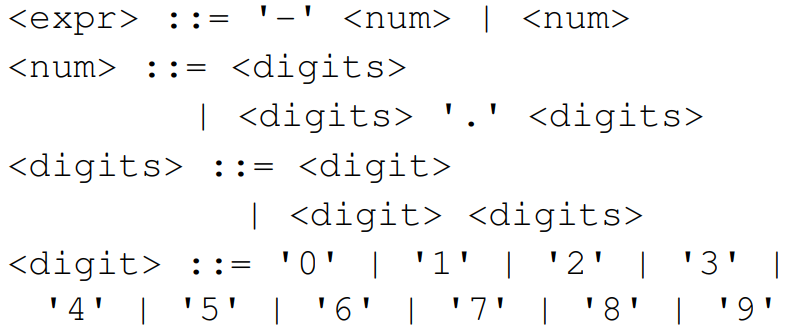
\includegraphics[scale=0.5]{images/BNF.PNG}
    \caption{BNF Notation Decimal Numbers}
    \label{fig:bnf}
\end{figure}

Niklaus Wirth started the early developments of EBNF which is an extension of BNF and make expressing grammars more convenient \cite{bnf_vs_ebnf}. One of the greatest improvements is the definition of the symbol occurrences (from 0 or more occurences). An example of the EBNF form for decimal numbers is presented on Figure XXXX.

\begin{figure}[H]
    \centering
    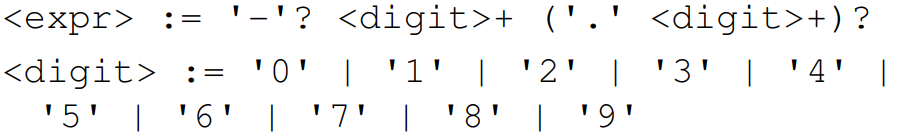
\includegraphics[scale=0.5]{images/EBNF.PNG}
    \caption{EBNF Notation Decimal Numbers}
    \label{fig:ebnf}
\end{figure}

EBNF is now widely used as the de-facto standard to define programming languages.\\

Context-free grammars rank as a Chomsky type 2 in Chomsky hierarchy. The Hierarchy of chomsky is defined as follows:

TABELA XXXXX



Language Recognition tools such as ANTLR contain two processes that work in sequence, lexing and parsing. The Lexer scans the input and produces the matching tokens, the parser then scans the tokens and produces the parsing result CITE XXXX.

its a lot easier to write a top-bottom grammar than a bottom-up one

a language is a set of production rules





%----------------------- Software testing ----------------------------
\section{Software testing}
\label{sec:software_testing}

The purpose of software testing activities is to verify that a system is operating according to predefined design and meets the customer needs.
Testing can occur on different levels 
\\
\textcolor{red}{
Notes:\\
what is the purpose of testing activities\\
who should be testing\\
who writes tests\\
why are tests so important ... (without tests the software would be prone to errors)\\
FALAR DO V-MODEL\\
introduzir paths and branchs
}


\subsection{Black-box testing}
\label{subsec:black-box testing}

Cause-Effect graph 


\section{Requirement Testing Tools}
\label{subsec:requirement_testing}

Cucumber\\
Cucumber is a tool that supports behaviour-driven development. It reads Test definitions and test steps written using the Gherkin language \cite{cucumber}.\\

Jest\\
Cypress\\

%----------------------- Software testing ----------------------------
\section{Related Works}
\label{sec:related_works}

Artigos\\

%----------------------- Current procedures ----------------------------
\section{Overview of the current industry procedures}
\label{sec:current_procedures}

This section presents the system testing activities in which critical software is involved.
The process begins when the rolling stock manufacturer receives a set of customer requirements commonly known as \textit{Business Requirements}. Aside from these requirements, there are the \textit{Rule Book} requirements which are documents that contain direct instructions to Railway staff, as well as the requirements from the \textit{standards} catalogues related to a Safety Integrity Level (SIL). SIL levels go from level 0 to level 4 according to the criticality of a system being SIL-4 systems less prone to fail. 

The concept of safety integrity was then taken up and adapted in the
various offshoot standards. For the railway domain, the concept of safety
integrity was taken up in the CENELEC EN 50126, EN 50128 and EN
50129 standards \cite{cenelec50128}.

The acceptable (or tolerable) risk is a value of a risk level arrived at by an
objective, deliberate decision. This threshold of acceptability is known as the
THR (Tolerable Hazard Rate). The THR is expressed as the probability of
occurrence of a failure, expressed in the form \[ 10^x \] per hour. When
identifying hazardous situations, it is crucial to assign them a THR, which
must be included in the specification \cite{cenelec50128}.

For the railway domain, Figure \ref{fig:sillevels} shows the link which exists between the
SIL and the THR. In fact, this table was introduced for railway signaling and
can be extended to all or part of the system \cite{cenelec50128}.

\begin{figure}[H]
    \centering
    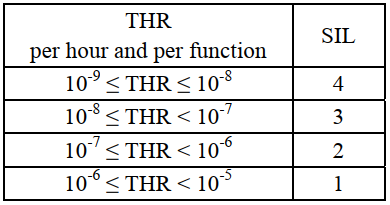
\includegraphics[scale=0.6]{images/SILlevels.PNG}
    \caption{SIL Table from CENELEC EN 50129}
    \label{fig:sillevels}
\end{figure}


There are several \textit{standards} catalogues applicable to the railway industry. The practices involved in the development of the software are mostly presented on BS EN 50126 \cite{en50126} and CENELEC 50128 \cite{cenelec50128}. BS EN 50126 is a standard that introduces the RAMS process, which is a process that characterises a system in terms of Reliability, Availability, Maintainability and Safety. The objective of the RAMS process described in this standard (BS EN 50126) is to ensure that all aspects of RAMS are covered in order to make provision for the safety of railway applications and for the avoidance of loss of their value \cite{en50126}. 

CENELEC 50128 specifies the process and technical requirements for the development of software for programmable electronic systems for use in railway control and protection applications. It is aimed at use in any area where there are safety implications. These systems can be implemented using dedicated microprocessors, programmable logic controllers, multiprocessor distributed systems, larger scale central processor systems or other architectures \cite{en50128_2}. 

The Functional Architecture team is responsible for the apportionment of the existing requirements as defined on section \textcolor{blue}{REF PARA O V-MODEL}. These existing requirements are usually derived into new architectural, performance, functional and sub-system requirements as seen on Figure \ref{fig:system_hierarchy}.\\

\begin{figure}[h]
    \centering
    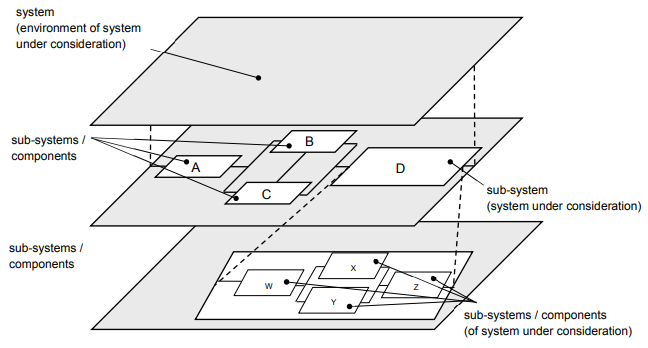
\includegraphics[width=\textwidth]{images/subsystem_reqs.PNG}
    \caption{System Hierarchy}
    \label{fig:system_hierarchy}
\end{figure}


The functional team, responsible of Functional requirements, needs to assure that these derived requirements satisfy the original customer requirements, are testable, coherent and non-contradictory. The development team writes software requirements derived from functional level and implements the software following the norm EN 61131 \cite{en61131}. To facilitate code safety, Ada language \cite{ada_book} and Misra-C \cite{misra_c} are also used at critical software in the area of Aerospace, Defense and Transportation (ADST).\\

The software is only uploaded to vehicle level once all previous tests pass under a simulated environment in the form of a \textit{Test Rack} (Figure \ref{fig:test_rack}) for SIL requirements, containing all the train equipment that compose the TCMS (Train Control and Management Systemm) like the Central Control Unit of the train. Some parts of the TCMS software, like the Passenger Information System are non-SIL, and are usually tested in a form of a virtual environment installed on the testers' computer. \\

\begin{figure}[h]
    \centering
    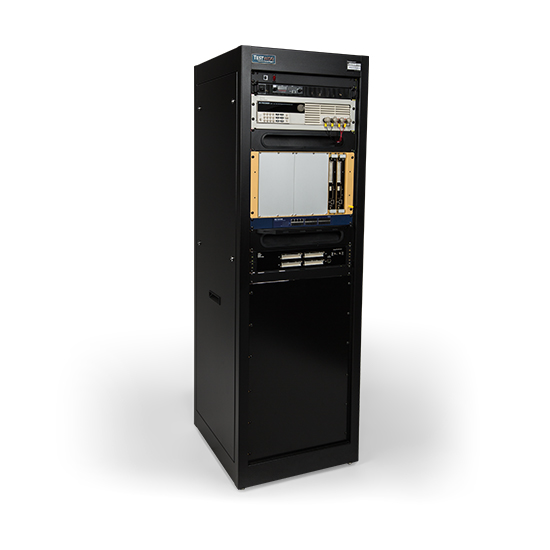
\includegraphics[scale=0.5]{images/testrack.jpg}
    \caption{Test Rack - Train Test Equipment}
    \label{fig:test_rack}
\end{figure}

The activity of testing relies on the interpretation of the software requirements stored on an IBM DOORS database by the manufacturer, and the verification if the system is behaving accordingly. To support the testing activities at system testing level, an Interface Control Document (ICD) is required. The purpose of the ICD is to support the information present on a requirement by mapping its conditions to one or more software signals, which are the internal logic of the Train Control and Management System (TCMS) and might act from a simple button press to the representation of the status of a train door.\\

The realisation of testing a requirement relies on the identification of software signals that represent the logic present on a requirement e.g. the command to open a train door, passenger emergency button, etc. and on the definition of the combination between the inputs and expected results in order to meet the requirement coverage criteria. This combination of test steps results in a test specification that can be converted into a test script using a test tool provided by the manufacturer. The test script is then loaded on the test tool which will then produce a test report file. Tests might by automatic or semi-automatic depending on the nature of the system. 


\section{Conclusions on state of the art}
\label{sec:sota_conclusions}

Alguns artigos lidos tentam chegar à interpretação de linguagem natural, que pode induzir em erro, ou definem uma linguagem natural controlada mas dependem de muitos inputs do utilizador, outros artigos pedem ao utilizador para atribuir significado às palavras na altura do processamento do requisito.

